
%(BEGIN_QUESTION)
% Copyright 2015, Tony R. Kuphaldt, released under the Creative Commons Attribution License (v 1.0)
% This means you may do almost anything with this work of mine, so long as you give me proper credit

A technician is troubleshooting a faulty optically-isolated TRIAC power switching circuit.  The solenoid valve is supposed to open up when the pushbutton switch is pressed and shut when the switch is released, but it remains open (passing liquid) no matter what state the switch is in.  A mechanic replaces the solenoid valve, thinking it is frozen open.  However, even the brand-new solenoid valve remains open and refuses to shut:

$$\includegraphics[width=15.5cm]{i03180x01.eps}$$

Leaving the switch in its normal (``unpressed'') position, the technician measures approximately 0.1 volts AC between test points TP5 and TP6, and 9 volts DC (normal for the battery) between test points TP1 and TP3.  Based on these voltage measurements, identify two possible faults (either one of which could account for the problem and all measured values in this circuit), and also identify two circuit elements that could not possibly be to blame (i.e. two things that you know {\it must} be functioning properly, no matter what else may be faulted).  The circuit elements you identify as either possibly faulted or properly functioning can be wires, traces, and connections as well as components.  Be as specific as you can in your answers, identifying both the circuit element and the type of fault.

\begin{itemize}
\item{} Circuit elements that are possibly faulted
\item{1.} 
\item{2.} 
\end{itemize}

\begin{itemize}
\item{} Circuit elements that must be functioning properly
\item{1.} 
\item{2.} 
\end{itemize}

\vfil 

\underbar{file i03180}
\eject
%(END_QUESTION)





%(BEGIN_ANSWER)

This is a graded question -- no answers or hints given!

%(END_ANSWER)





%(BEGIN_NOTES)

The fact that the TRIAC is only dropping 0.1 volt AC, coupled with the symptom of the solenoid valve remaining open when it shouldn't be, tells us the optocoupler is passing AC power to the solenoid valve when it shouldn't be.  Therefore, we need to look for faults that would cause the TRIAC to pass power at all times.

\begin{itemize}
\item{} Circuit elements that are possibly faulted
\item{1.} shorted TRIAC 
\item{2.} shorted pushbutton switch
\end{itemize}

\begin{itemize}
\item{} Circuit elements that must be functioning properly
\item{1.} AC power source
\item{2.} 9 volt battery
\end{itemize}

%INDEX% Troubleshooting review: electric circuits

%(END_NOTES)


